\pagebreak
\section{Sensoren}\label{sec:Sensoren}

% Hinweis auf C-Code, Verweise auf Kapitel von olliver, nur Besonderheiten hier erwähnt

% Überall noch Daten aus Präsentation einbringen, eventuell kleine Tabellen, nicht zwingend

% Verweis auf Strom und Spannungsmessung (das haben wir schon, Rest kommmt JETZT)

\subsection{Kompassmodul QMC5883L}
Als Kompass dient uns der \textbf{QMC5883L}. Das Bauteil ist zwar mit \textbf{HMC5883L} beschriftet, verbaut ist aber ein \textbf{QMC5883L}. Überprüfen lässt sich dies über ein Auslesen der Registeradresse, welche den Wert \textit{0x0D} statt wie erwartet \textit{0x3D/0x3C} zurückgibt.

Verwendet wird er, um die Ausrichtung der Wetterstation gen Norden zu messen (s. Kap.~\ref{sec:ausrichtung des Solarpanels}). Diese Information wird benötigt, um das Solarpanel korrekt zur Sonne auszurichten zu können. 

Auf die Software zu dem Kompassmodul wird in Kapitel \ref{ssec:QMC5883L} eingegangen.

\subsubsection{Montage}
Das Kompassmodul hat 5 Anschlüsse, von denen vier verwendet werden: V\textsubscript{CC}, GND, SDA und SCL. Der fünfte Anschluss wird nur bei einer häufigen Datenübertragung benötigt. Er sendet die Information, dass Daten zum Abruf bereit stehen. Dargestellt ist die Verschaltung in Abbildung~\ref{fig:QMC5883L_Plan}.

\begin{figure}[H]
  \centering
  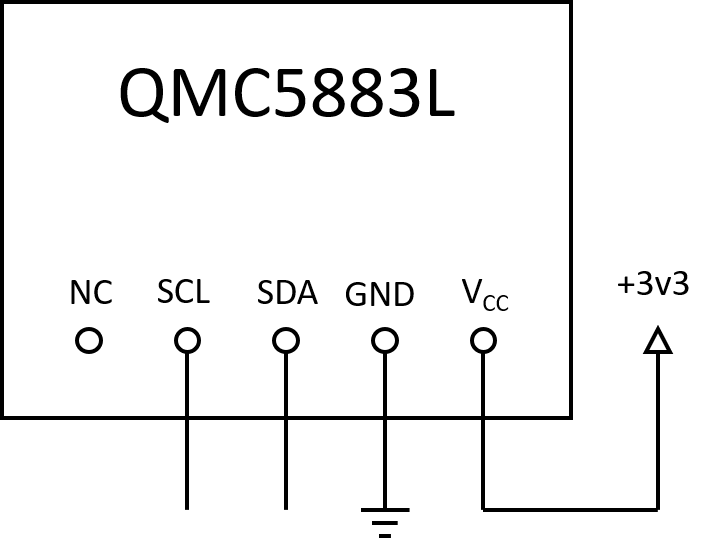
\includegraphics[width=0.4\textwidth]{./img/QMC5883L_Plan.png}
  \caption{Verschaltung des QMC5883L}\label{fig:QMC5883L_Plan}
\end{figure}

Um den Sensor fest zu verbauen, aber gleichzeitig ein Austauschen möglich zu machen, wurde eine Lochrasterplatine zugeschnitten und dann mit entsprechenden Steckverbindungen (\textit{male} für das Kabel, \textit{female} für den Sensor) ausgestattet. Anschließend wurde diese in einem Deckel der Nebengehäuse (s. Kap.~\ref{sec:ge_neben}) eingeklebt. Als letzten Schritt musste nur noch ein Kabel mit 4 Adern gefertigt werden, um die Lochrasterplatine mit dem Board zu verbinden.

Da der Sensor das Magnetfeld misst, muss dieser zudem entfernt von der Windfahne und dem Anemometer platziert werden, da beide mit magnetischen Bauteilen arbeiten. Andernfalls könnte es zu Fehlmessungen kommen. Umgesetzt wurde dies so, dass an der einen Stütze des Solarpanels das Kompassmodul und an der anderen die Windfahne, das Anemometer und das gegenüber magnetischen Beeinflussungen relativ unempfindliche GPS-Modul angebracht wurden (s. Abb.~\ref{fig:Montage_Kompass_Wind}).

\begin{figure}[H]
 \centering
  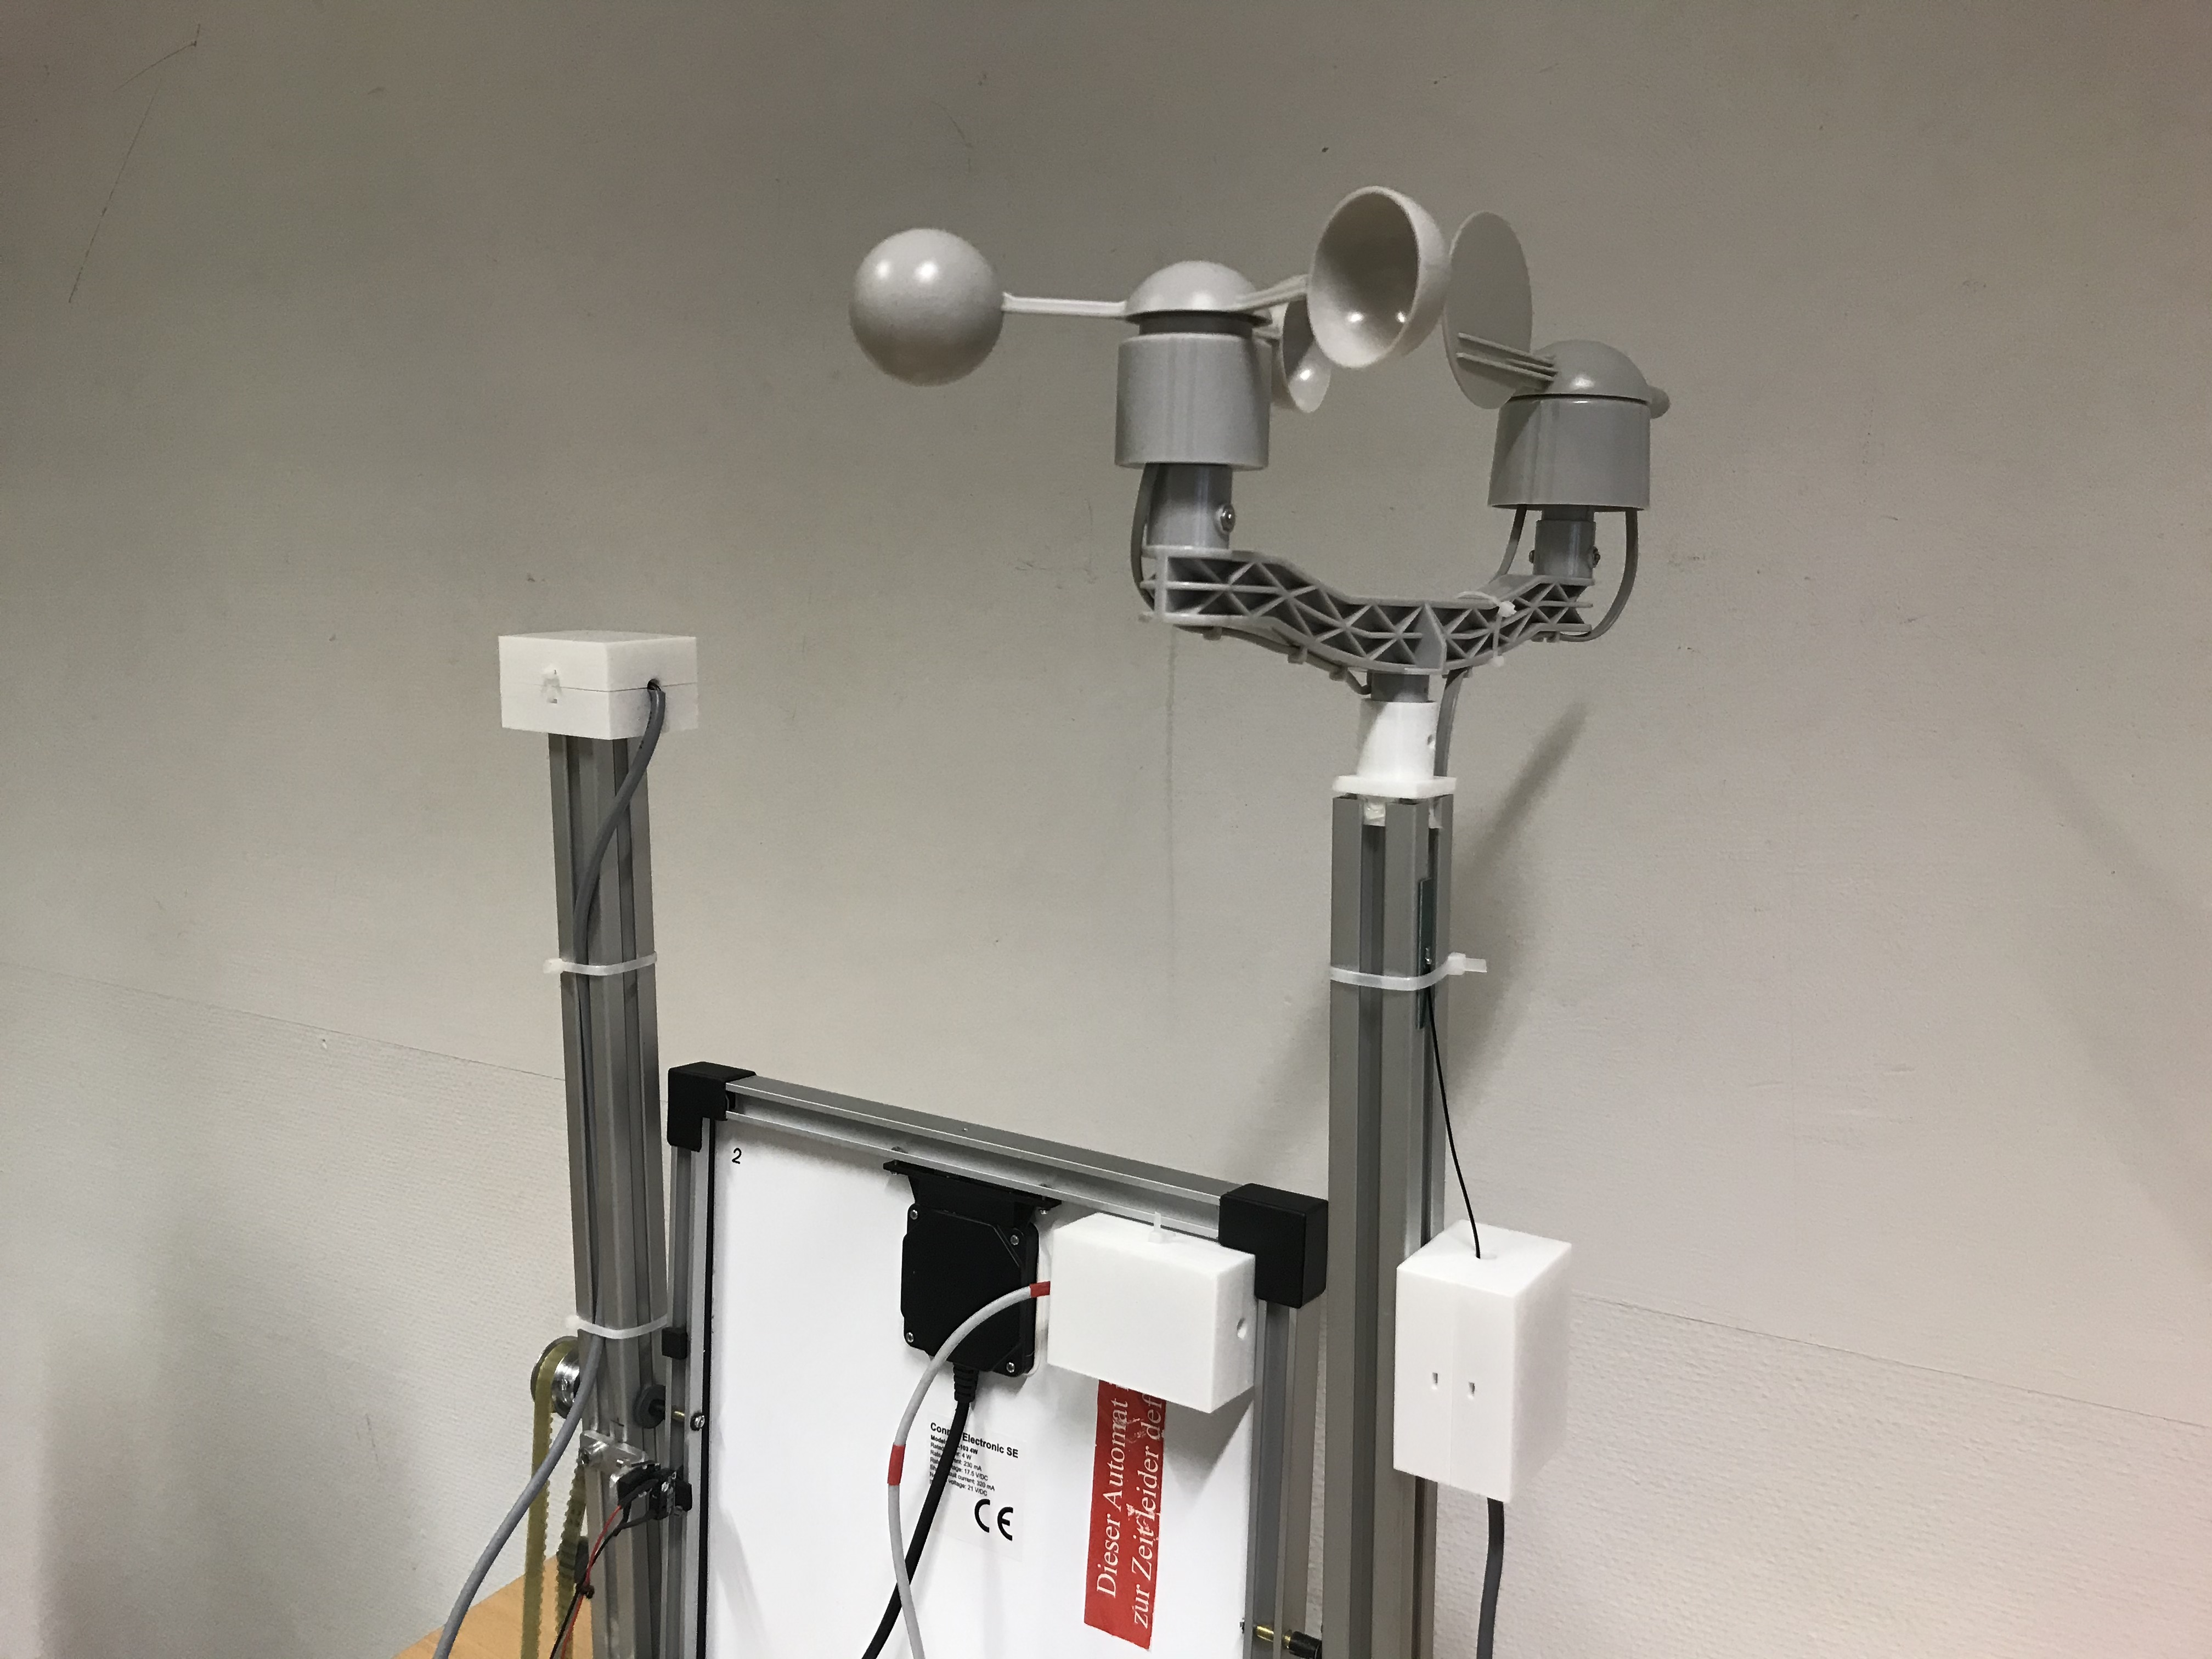
\includegraphics[width=0.8\textwidth]{./img/Montage_Kompass_Wind.JPG}
  \caption{Platzierung des Kompassmoduls auf der linken Stütze und Windfahne, Anemometer und GPS-Modul auf der rechten Stütze. An der Rückseite des Solarpanels befindet sich der Neigungssensor.}\label{fig:Montage_Kompass_Wind}
\end{figure}

\subsection{NEO-6M GPS-Modul} % richtiges Datenblatt finden und Werte einsetzen
Um den Standort des Geräts zu bestimmen und so die Berechnung der korrekten Auslenkung des Solarpanels auf Grund des Standorts zu ermöglichen, musste ein GPS-Modul genutzt werden. Wir haben uns für den \textbf{NEO-6M} von der Firma \textbf{u-blox} entschieden. Er ermöglicht eine Bestimmung der aktuellen Position bei einer Abweichung von \SI{2.5}{\meter} \cite{neo_GPS}. Das Modul wird mittels \textit{USART} angesprochen, die verwendete Software wird in Kapitel~\ref{ssec:GPS} genauer erklärt.

\subsubsection{Montage}
Da das GPS-Modul in Einheit mit einer Antenne funktioniert, musste das Modul entfernt von der Elektronik und damit außerhalb des Gehäuses platziert werden. Dazu bot sich an, das GPS-Modul an der zweiten Stütze des Solarpanels zu platzieren. Das Modul wurde dafür ebenso in einem Nebengehäuse untergebracht (s. Kap.~\ref{sec:ge_neben}). Die Antenne des Moduls wurde dabei mittels Kabelbinder an der Stütze angebracht. Dieses Vorgehen war einer dauerhaften Anbringung, etwa durch Kleber, vorzuziehen, da die Bauteile so leichter ausgetauscht werden können. Zu sehen ist dies in Abbildung~\ref{fig:Montage_Kompass_Wind}.

Das Modul hat fünf Anschlüsse V\textsubscript{CC}, GND, TXD, RXD und PPS. Der PPS-Anschluss blieb unverbunden (s. Abb.~\ref{fig:NEO-6_Plan}).

\begin{figure}[H]
  \centering
  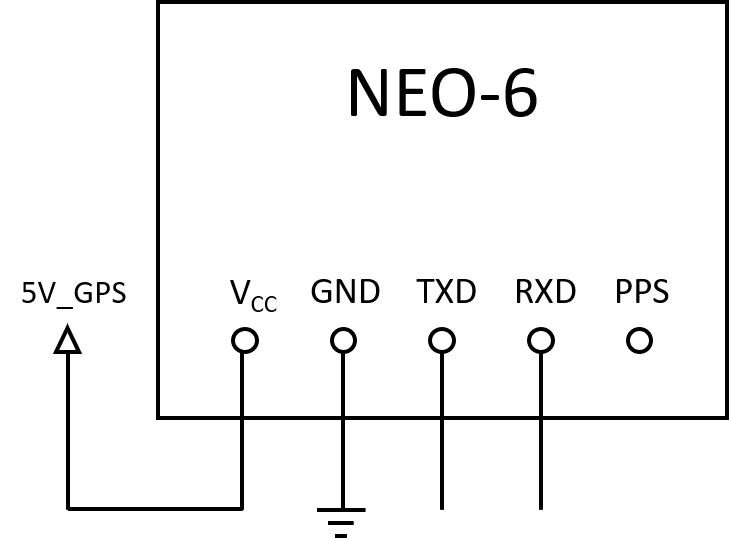
\includegraphics[width=0.4\textwidth]{./img/NEO-6_Plan.png}
  \caption{Verschaltung des NEO-6}\label{fig:NEO-6_Plan}
\end{figure}

\subsection{Anemometer und Windfahne: SEN-08942}
% Vorgänger wegen seriell und so doof
% neues Modell mit Doku, andernfalls reverse Ingeneering
% Funktion
Bei unseren Vorgängern waren diese Sensoren ein Problem, da sie keine Dokumentation zu einer seriellen Kommunikation hatten und zunächst aufwändig mittels Reverse-Engineering herausfinden mussten, wie sie den Sensor zu verwenden hatten. Bei diesem Projekt entschied man sich daher für einen neuen Sensor. Die Suche wurde dadurch erschwert, dass Anemometer und Windfahnen oft in einem System mit einer schon vorhandenen Wetterstation angeboten werden. Die Entscheidung fiel schlussendlich zu Gunsten des \textbf{SEN-08942}. Dieses System besteht aus einer Windfahne, einem Anemometer und einem Regenmesser.

Das Anemometer misst den Wind in dem es bei jeder Umdrehung einen Impuls ausgibt. In dem rotierendem System ist ein Magnet verbaut der an einem Schalter vorbei rotiert und so den Impuls verursacht. Ein Impuls pro Sekunde entspricht dabei laut Datenblatt einer Windgeschwindigkeit von \SI{2.4}{\km\per\hour} \cite{argent_data_systems}.

Die Funktion der Windfahne basiert darauf, dass 8 Schalter, jeweils mit einem anderen Widerstand verbunden, verbaut sind (s. Abb~\ref{fig:Wind_Plan}). Je nach Position der Fahne sind bis zu zwei Schalter geschlossen. Mit einem externen Widerstand kann dann ein Spannungsteiler genutzt werden, um die zu messende Spannung in eine Windrichtung überführen. 

\begin{figure}[H]
  \centering
  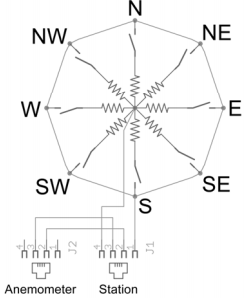
\includegraphics[width=0.5\textwidth]{./img/Wind_Plan.png}
  \caption{Aufbau der Windfahne und Anschluss an das Board\cite{ds_wind}}\label{fig:Wind_Plan}
\end{figure}

Für einen Spannungsteiler mit einem externen Widerstand von \SI{10}{\kilo\ohm} ergeben sich die Werte aus Abbildung~\ref{fig:Wind_Werte}.

\begin{figure}[H]
  \centering
  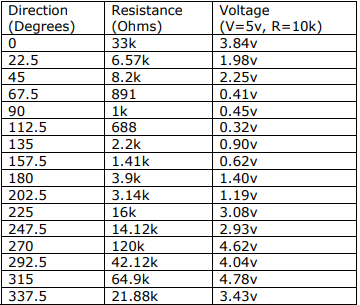
\includegraphics[width=0.6\textwidth]{./img/Wind_Werte.png}
  \caption{Beispielwerte der Windfahne mit \SI{10}{\kilo\ohm} \citep{argent_data_systems}}\label{fig:Wind_Werte}
\end{figure}

Der Regenmesser wurde im vorliegenden Aufbau nicht verwendet. Die Software zum Auslesen der beiden Sensoren findet sich in Kapitel~\ref{ssec:Wind}.

\subsubsection{Montage}
% Position
Die Windfahne und das Anemometer wurde auf der mitgelieferten Strebe befestigt. Mit Hilfe des gedruckten Adapters (s. Kap.~\ref{sec:ge_adapt}) wurden die beiden Sensoren, wie in Abbildung~\ref{fig:Montage_Kompass_Wind} zu sehen, auf einer der Stützen des Solarpanels befestigt.

Die Anschlüsse wurden wie in Abbildung~\ref{fig:Wind_Plan} vorgenommen. Das mitgelieferte RJ 11 Kabel wurde direkt an das Board angeschlossen. Pin 2 und 3 sind dabei mit GND verbunden. PIN 4 wurde mit \textit{Tim3\_ANEM\_CH1} und PIN 5 mit \textit{ADC1\_WV\_IN16} verbunden. PIN 5 wurde zudem über einen Widerstand von \SI{10}{\kilo\ohm} mit der $+3v3$ Leitung verbunden.

\subsection{Neigungssensor MPU6050}
% Zweck, Bestimmung Neigung des Panels, Feedback für Motor
Der Neigungssensor soll genutzt werden, um die Neigung des Solarpanels überprüfen zu können und so eine optimale Ausrichtung zu ermöglichen. Bei dem verwendeten Sensor handelt es sich um einen 6-Achsen Bewegungssensor, der ein 3-Achsen Gyroskop mit einem 3-Achsen Beschleunigungssensor verbindet. Er kann mittels I\textsuperscript{2}C-Schnittstelle angesprochen werden. \cite{ds_mpu6050}

Auf die Software wird in Kapitel~\ref{ssec:MPU6050} eingegangen.

\subsubsection{Montage}
In Abbildung~\ref{fig:MPU6050_Plan} sieht man, wie der Sensor verbunden ist. Er wurde wie das GPS-Modul und der Kompass auf eine Lochrasterplatine gesteckt und dann in einem der drei Nebengehäuse untergebracht. Anschließend wurde das Gehäuse mittels beidseitigem Klebeband hinten am Solarpanel angebracht (s. Abb.~\ref{fig:Montage_Kompass_Wind}).
\begin{figure}[H]
  \centering
  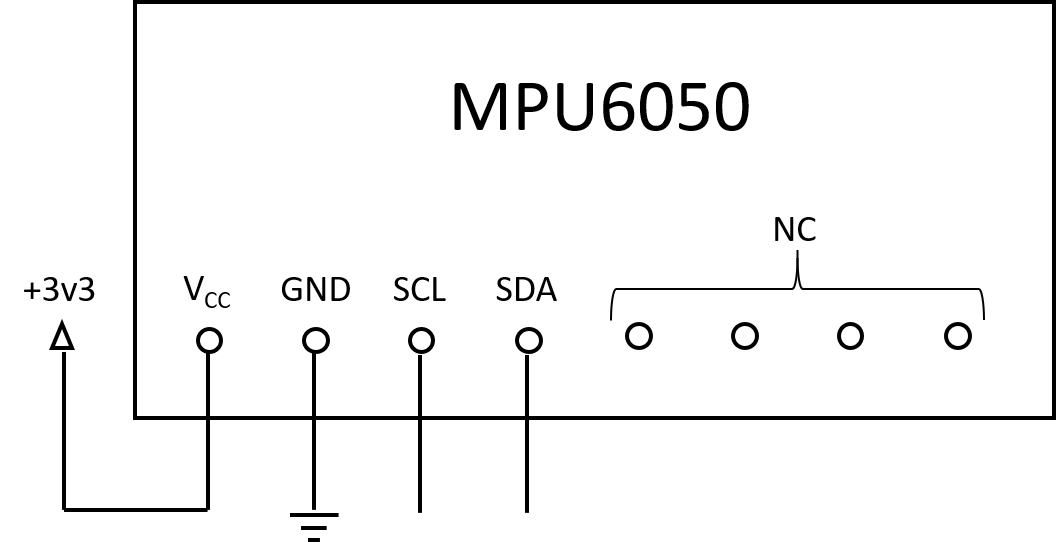
\includegraphics[width=0.6\textwidth]{./img/MPU6050_Plan.png}
  \caption{Verschaltung des MPU6050}\label{fig:MPU6050_Plan}
\end{figure}

\subsection{BME280}
% Zweck, Genauigkeit, Arbeitsbereich
Der \textbf{BME280} ist ein Sensor, der Luftfeuchtigkeit, Luftdruck und Temperatur aufnehmen kann. Hergestellt wird er von der Firma \textbf{BOSCH}. Angesteuert wird er über die I\textsuperscript{2}C-Schnittstelle. Die Luftfeuchtigkeit wird mit einer Genauigkeit von $\pm3\%$ bestimmt. Je nach Umgebungstemperatur kann der Luftdruck mit einer Genauigkeit von $\pm1$ bis $\pm1.7$~hPa genau bestimmt werden. Die Genauigkeit der Temperatur geht von minimal $\pm$\SI{0.5}{\celsius} bis $\pm$\SI{1.5}{\celsius}. Zudem bietet der Sensor die Möglichkeit, ihn in mehreren Betriebsmodi zu betreiben. So kann er etwa für längere Zeit im Sleepmodus gehalten werden und wird erst zur Messwertabfrage geweckt, was den Stromverbrauch reduziert.\cite{ds_bme280}

Die Software zu dem Sensor wird in Kapitel~\ref{ssec:BME280} genauer erläutert.

\subsubsection{Montage}
% Wo ist der? Im Gehäuse? Bild!
Der Sensor wurde direkt auf dem Board angebracht. Da das Hauptgehäuse (s. Kap.~\ref{sec:ge_haupt}) offen ist, wird die Umgebungsluft ungehindert an den Sensor gelangen. Die Anschlüsse können aus Abbildung~\ref{fig:BME280_Plan} entnommen werden.

\begin{figure}[H]
  \centering
  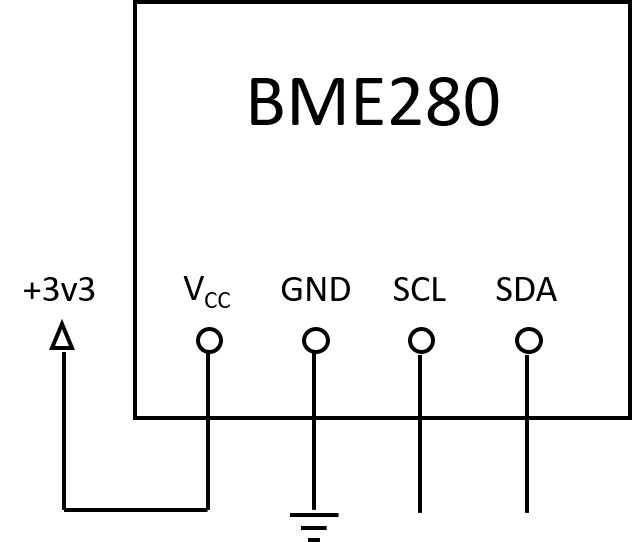
\includegraphics[width=0.4\textwidth]{./img/BME280_Plan.png}
  \caption{Verschaltung des BME280}\label{fig:BME280_Plan}
\end{figure}

\subsection{Anschlagssensor}
% Zweck, Positionierung Panel, noch von Vorgängern, Schutz Motor und Teile. Funktion
Um den Motor, der für die Rotation des Solarpanels zuständig ist, vor Schäden durch Überdrehen zu schützen, wurden die von unseren Vorgängern am Aufbau befestigten Anschlagssensoren genutzt. Diese beiden Sensoren sitzen nahe der Rotationsachse des Panels Rauf der Rückseite des Aufbaus. Bei Drehen des Solarpanels auf Anschlag kontaktiert einer der Sensoren und gibt ein Signal an den Mikrocontroller weiter. Software-seitig wird nun der Motor ausgeschaltet und dient zunächst als Notaus.

Des Weiteren können die Anschlagssensoren zur Kalibrierung der Stellung des Solarpanels verwendet werden.

\subsubsection{Montage}
% an Achse des Panels

% Verkabelung erklären
Wie schon erwähnt sind die beiden Sensoren achsennah montiert. Angeschlossen sind die beiden Sensoren mit drei Kabeln: GND, einer Versorgungsspannung und einer Signalleitung.
